\documentclass[12pt,a4paper]{ctexart}
\usepackage{geometry}
\geometry{left=2.5cm,right=2.5cm,top=2.0cm,bottom=2.5cm}
% \usepackage[english]{babel}
\usepackage{amsmath,amsthm}
\usepackage{amsfonts}
\usepackage[longend,ruled,linesnumbered]{algorithm2e}
\usepackage{fancyhdr}
\usepackage{array}
\usepackage{listings}
\usepackage{color}
\usepackage{graphicx}
\usepackage{minted}
\usepackage{float}
\usepackage[defaultmono]{droidsansmono}

\graphicspath{{pics/}}
\ctexset{today=small}
\definecolor{codebg}{rgb}{0.95,0.95,0.95}

\input{personal_info/info.tex}

\begin{document}
    \begin{titlepage}
        \heiti
        \vspace*{64pt}
        \begin{center}
            \fontsize{48pt}{0} 算法设计与分析\\
            \vspace*{36pt}
            \fontsize{48pt}{0}{实\quad 验\quad 报\quad 告}\\
            \vspace*{48pt}
            \LARGE(2021\~{}2022 学年度\qquad 第 3 学期)\\
            \vspace*{48pt}
        
            \LARGE 实验名称\ \ \underline{\makebox[200pt]{\ExamTitle}}\\
            \LARGE 实验地点\ \ \underline{\makebox[200pt]{\ExamAddr}}\\
            \LARGE 实验日期\ \ \underline{\makebox[200pt]{\today}}\\
            \LARGE 学生姓名\ \ \underline{\makebox[200pt]{\MyName}}\\
            \LARGE 学生学号\ \ \underline{\makebox[200pt]{\MySID}}\\
            \LARGE 指导教师\ \ \underline{\makebox[200pt]{\TeacherName}}\\
            \vspace*{48pt}
            
            \LARGE 东南大学\quad  计软智学院 \quad 制
        \end{center}
    \end{titlepage}

\title{
  {\heiti \textbf{实验三\ 动态规划}
    \footnote{要求:1、分析题请用书面化语言给出详细分析过程。2、实验请统一使用ex0*-学号-姓名的命名格式,latex版本请附上源代码并打包提交。}
    }
}
\date{}

\maketitle

\section*{\bf \color{black}{一、实验目的及意义}}
\noindent
\begin{enumerate}
	\item[(1)]  掌握动态规划算法的基本思想、求解问题的基本步骤;
	\item[(2)]  掌握动态规划算法的时间复杂度;
	\item[(3)]  学会利用动态规划算法解决实际问题。
\end{enumerate}

\vspace{5pt}

\section*{二、实验内容与结果}
\subsection*{题目1:收集骨头}
\paragraph{题目内容}
\subparagraph{题目描述}
\begin{itemize}
    \item 有一个骨头收藏家,这个人喜欢收集各种各样的骨头,比如狗的,牛的。该收藏者有一个体积为$V$的大袋子,在他收集的旅途中有很多骨头,不同的骨头有不同的价值和体积,现在给每个骨头标定一个价值,你能计算出该收藏者能得到的总价值的最大值吗?
\end{itemize}

\subparagraph{输入格式}
    \begin{itemize}
        \item 第一行包含2个正整数$N , V (1 \leq N \leq 1000 , 1 \leq V \leq 1000 )$,表示骨头数量以及背包容量; 
        \item 第二行包含N个整数,表示每个骨头的价值;
        \item 第三行包含N个整数,表示每个骨头的体积。
    \end{itemize}
\subparagraph{输出格式}
    \begin{itemize}
        \item 输出一个整数,表示能得到的最大价值。(该值小于$2^{31}$)
    \end{itemize}

\subparagraph{输入输出样例}
如下表
    \begin{figure}[h]
        \centering
        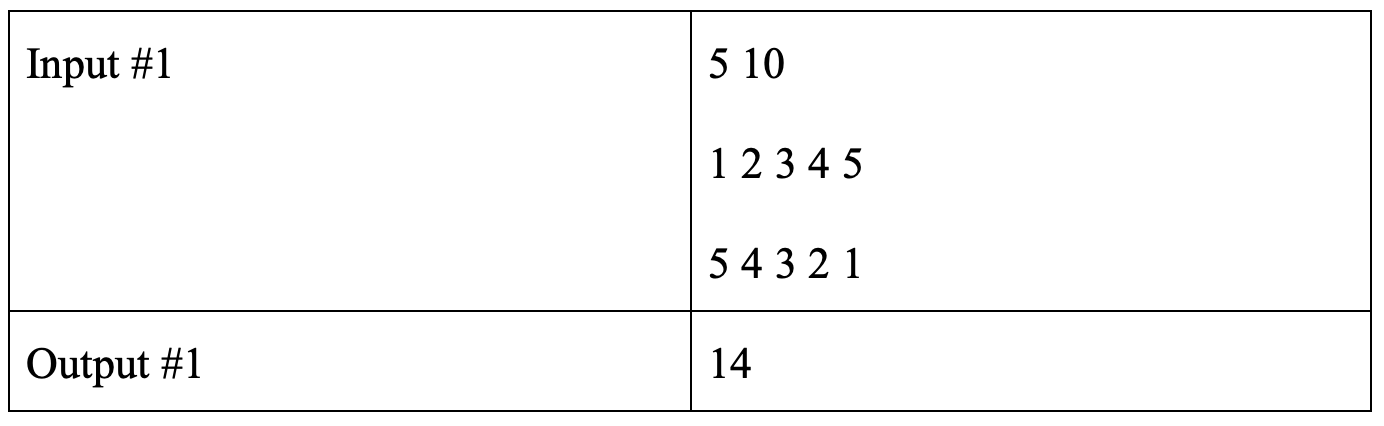
\includegraphics[width=0.80\textwidth]{q1_iodata.png}
    \end{figure}

\vspace{5pt}

\paragraph{实验环境}
\begin{itemize}
    \item 程序设计语言:C++
    \item 编程环境:
    \begin{itemize}
        \item 编辑器:Visual Studio Code (1.67.0)
        \item 编译器:g++ (GCC) 11.2.0
        \item 操作系统:ArchLinux 5.17.5-zen1-1-zen (64-bit)
    \end{itemize}
\end{itemize}

\vspace{5pt}

\paragraph{解答} 时间复杂度:$\Theta(NV)$

源码:
\inputminted[bgcolor=codebg,frame=lines,autogobble,linenos=true,breaklines]{cpp}{src/t2.cpp}

\vspace{5pt}

\paragraph{实验结果}AC (9ms/864.00KB)


\subsection*{题目2:打家劫舍}
\paragraph{题目内容}
\subparagraph{题目描述}
\begin{itemize}
    \item 你是一个专业的小偷,计划偷窃沿街的房屋,每间房内都藏有一定的现金。这个地方所有的房屋都 围成一圈 ,这意味着第一个房屋和最后一个房屋是紧挨着的。同时,相邻的房屋装有相互连通的防盗系统,如果两间相邻的房屋在同一晚上被小偷闯入,系统会自动报警 。
    \item 给定一个代表每个房屋存放金额的非负整数数组,计算你在不触动警报装置的情况下 ,今晚能够偷窃到的最高金额。

\end{itemize}

\subparagraph{输入格式}
    \begin{itemize}
        \item 第一行输入房屋数量N;
        \item 第二行输入长度为N的数组,表示房屋中存放的金额。
    \end{itemize}

\subparagraph{输出格式}
    \begin{itemize}
        \item 输出能偷窃到的最高金额。
    \end{itemize}
    
\subparagraph{输入输出样例}
如下表
    \begin{figure}[h]
        \centering
        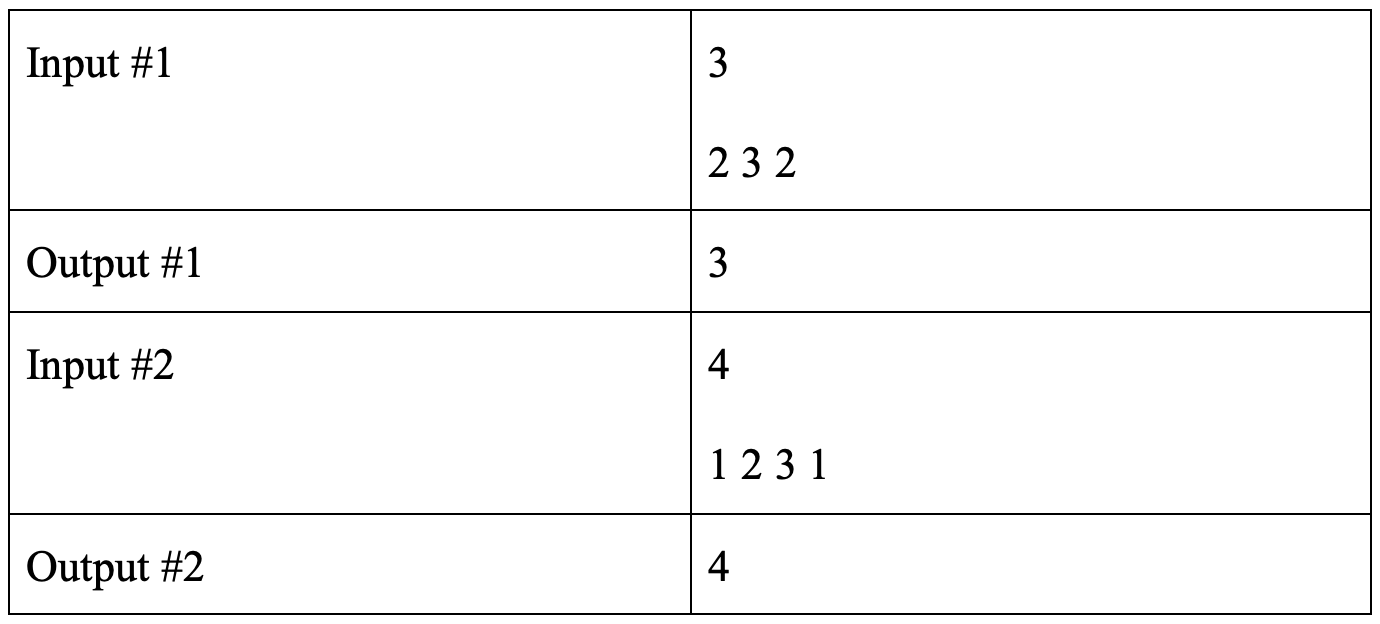
\includegraphics[width=0.80\textwidth]{q2_iodata.png}
    \end{figure}


\vspace{5pt}

\paragraph{实验环境}
\begin{itemize}
    \item 程序设计语言:C++
    \item 编程环境:
    \begin{itemize}
        \item 编辑器:Visual Studio Code (1.67.0)
        \item 编译器:g++ (GCC) 11.2.0
        \item 操作系统:ArchLinux 5.17.5-zen1-1-zen (64-bit)
    \end{itemize}
\end{itemize}

\vspace{5pt}

\paragraph{解答}时间复杂度:$\Theta(N)$

源码:
\inputminted[bgcolor=codebg,frame=lines,autogobble,linenos=true,breaklines]{cpp}{src/t1.cpp}

\vspace{5pt}

\paragraph{实验结果}AC (6ms/692.00KB)

\vspace{5pt}


\subsection*{题目3:纸牌游戏}
\paragraph{题目内容}
\subparagraph{题目描述}

\begin{itemize}
    \item 有N张扑克牌(全是1到9的数字牌),洗牌后,将所有牌面亮出摊成一个扇形,甲和乙轮流抽牌,每次只能从牌顶或牌底抽一张,放入手中。轮流抽完所有牌后,累计手中牌数字之和更大的人获胜。
    \item 给定一个表示分数的数组,预测玩家甲是否会成为赢家。你可以假设每个玩家的玩法都会使他的分数最大化。
\end{itemize}

\subparagraph{输入格式}
    \begin{itemize}
        \item 第一行输入纸牌张数N,即数组大小;
        \item 第二行输入长度为N的数组,表示纸牌牌面。
    \end{itemize}

\subparagraph{输出格式}
    \begin{itemize}
        \item 输出一行,玩家甲能否获胜,True或False。
    \end{itemize}
    

\subparagraph{输入输出样例}
如下表
    \begin{figure}[h]
        \centering
        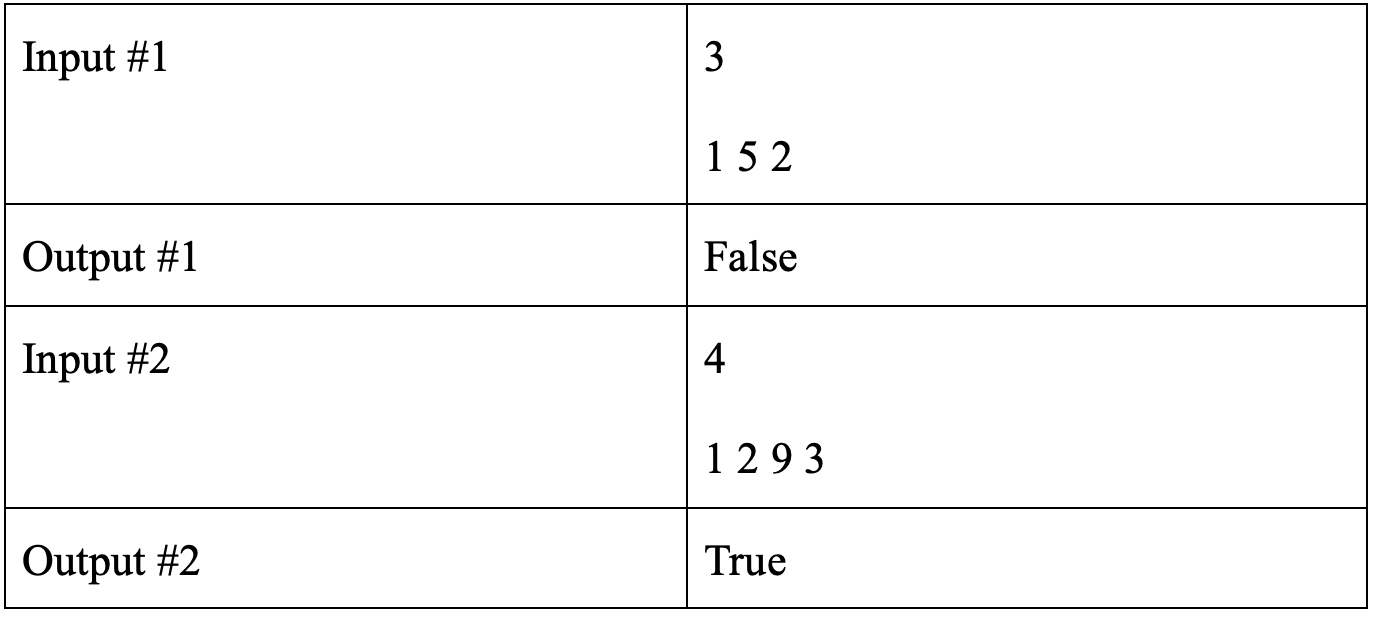
\includegraphics[width=0.80\textwidth]{q3_iodata.png}
    \end{figure}

\vspace{5pt}

\paragraph{实验环境}
\begin{itemize}
    \item 程序设计语言:C++
    \item 编程环境:
    \begin{itemize}
        \item 操作系统:ArchLinux 5.17.5-zen1-1-zen (64-bit)
        \item 编辑器:Visual Studio Code (1.67.0)
        \item 编译器:g++ (GCC) 11.2.0
    \end{itemize}
\end{itemize}

\vspace{5pt}

\paragraph{解答}时间复杂度:$\Theta(N^2)$

源码:
\inputminted[bgcolor=codebg,frame=lines,autogobble,linenos=true,breaklines]{cpp}{src/t3.cpp}

\vspace{5pt}

\paragraph{实验结果}AC (13ms/808.00KB)


\vspace{5pt}





\section*{三、心得体会}
\begin{enumerate}
    \item 前两题比较基础,没什么好讲的,除了第二题用了滚动数组,并且一部分输入可以不需要保存;
    \item 第三题通过活用 C++ 的语言机制(位运算和 Lambda 表达式)提高代码复用,在略微降低可读性的同时大幅度降低了代码长度;
    \begin{itemize}
        \item 第 5---10 行中的定义便是此种用法。其中,索引为 0 时取出的值为乙的策略,为 1 时取出的值为甲的策略;
        \item 第 24 行中的 \mintinline{cpp}{n & 1}:通过观察,可以得出当抓取最后一张牌时是甲的回合,当且仅当 $n$ 是奇数(\mintinline{cpp}{n & 1} 的值为 1);
        \item 第 30---31 行中的 \mintinline{cpp}{(i ^ n ^ 1) & 1}:在牌堆剩余 $i$ 张牌时,若 $i$ 与 $n$ 的奇偶性相同,则此时为甲的回合,否则为乙的回合。此表达式即为对以上表述的判断;
    \end{itemize}
    \item 第三题的思想似乎有一个所谓的``名字'':min-max 对抗搜索?不过本题相对简单,直接可以用逆向循环来代替搜索过程。
\end{enumerate}

\end{document} 
